%% Shared by main.tex (the paper you write) and draft.tex (the reference draft).
%% Format: the ICML 2026 kit, two columns, Times text and Computer Modern math. Page geometry, fonts and spacing
%% come from the kit and are never changed here. The kit is the provisional choice until the venue is decided:
%% for a journal (e.g. PRX Intelligence, revtex two-column), only this file and the \twocolumn[...] block in the
%% two main files change.

\usepackage{microtype}
\usepackage{graphicx}
\usepackage{booktabs}
\usepackage{xcolor}
\usepackage{hyperref}
\usepackage{tikz}
\usetikzlibrary{arrows.meta,calc,positioning}
\newcommand{\theHalgorithm}{\arabic{algorithm}}

% preprint: author names shown, footer "Preprint. <date>" (arXiv first, venue later).
% Anonymous submission: \usepackage{icml2026}.  Camera-ready: \usepackage[accepted]{icml2026}.
\usepackage[preprint]{icml2026}

\usepackage{amsmath}
\usepackage{amssymb}
\usepackage{mathtools}
\usepackage[capitalize,noabbrev]{cleveref}

\graphicspath{{figures/}}

%% ---------------------------------------------------------------- figures
%% Every plot is drawn at its printed size: 3.25 in for one column, 6.75 in for the full width (figure*).
%% Include them WITHOUT a width, so that the axis labels stay at the body's 10 pt:
%%     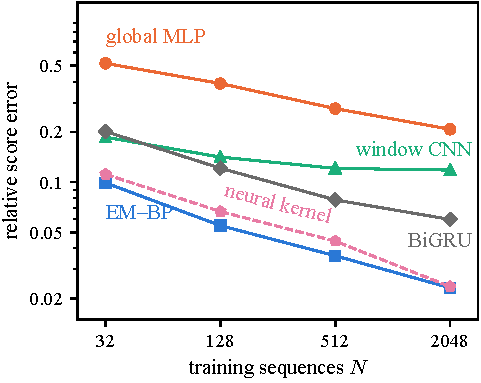
\includegraphics{fig_value_of_structure}
%% The plots and their style (box on all four sides, no grid, minor ticks, log scales, markers for measurements and
%% lines for closed forms) are made by tools/paper_figs/make_paper_figures.py in the research repository; see README.md.
%% The two diagrams are TikZ, \input from figures/*.tikz, so they use the body font and can be edited here.

%% ---------------------------------------------------------------- notation
\newcommand{\E}{\mathbb{E}}
\newcommand{\Normal}{\mathcal{N}}
\newcommand{\Kt}{K_\theta}
\newcommand{\dd}{\mathrm{d}}
\newcommand{\Dt}{\Delta_t}
\newcommand{\Ng}{N_g}

%% ---------------------------------------------------------------- writing aids
%% \note{...}    grey guidance text: what goes here, what Jerome asked for. Hide them all with \shownotesfalse.
%% \pending{...} a result that is not in yet (a run still on the cluster). Shown in orange so none is forgotten.
\newif\ifshownotes \shownotestrue
\definecolor{notegrey}{gray}{0.45}
\definecolor{pendingorange}{HTML}{C0501F}
\newcommand{\note}[1]{\ifshownotes{\color{notegrey}\itshape [#1]}\fi}
\newcommand{\pending}[1]{{\color{pendingorange}[pending: #1]}}
